\textcolor{prime}{\textsf{Findings}} \\
\begin{itemize}
\item When we only use the first term of the heuristic, (figure~\ref{fig:woheu}),  the system can leave a trot gait and quickly becomes unstable at higher amplitude disturbances.

\item When we use both terms of the heuristic, (figure~\ref{fig:wheu}), the system can reject higher amplitude disturbances because it is able to maintain a trot gait. 

\item System can still be forced to leave a trot gait if disturbance is large enough
\end{itemize}

\vspace{2EX}
\textcolor{prime}{\textsf{Future Work}} \\
\begin{itemize}
	\item Test the controller on a real robot to verify its robustness given:
	\begin{itemize}
		\item motor dynamics
		\item waves produced by feet
		\item sensor noise
	\end{itemize}
\end{itemize}

\vspace{2EX}
\begin{figure}[h]
\centering
\begin{subfigure}[t]{0.47\textwidth}
    \centering
    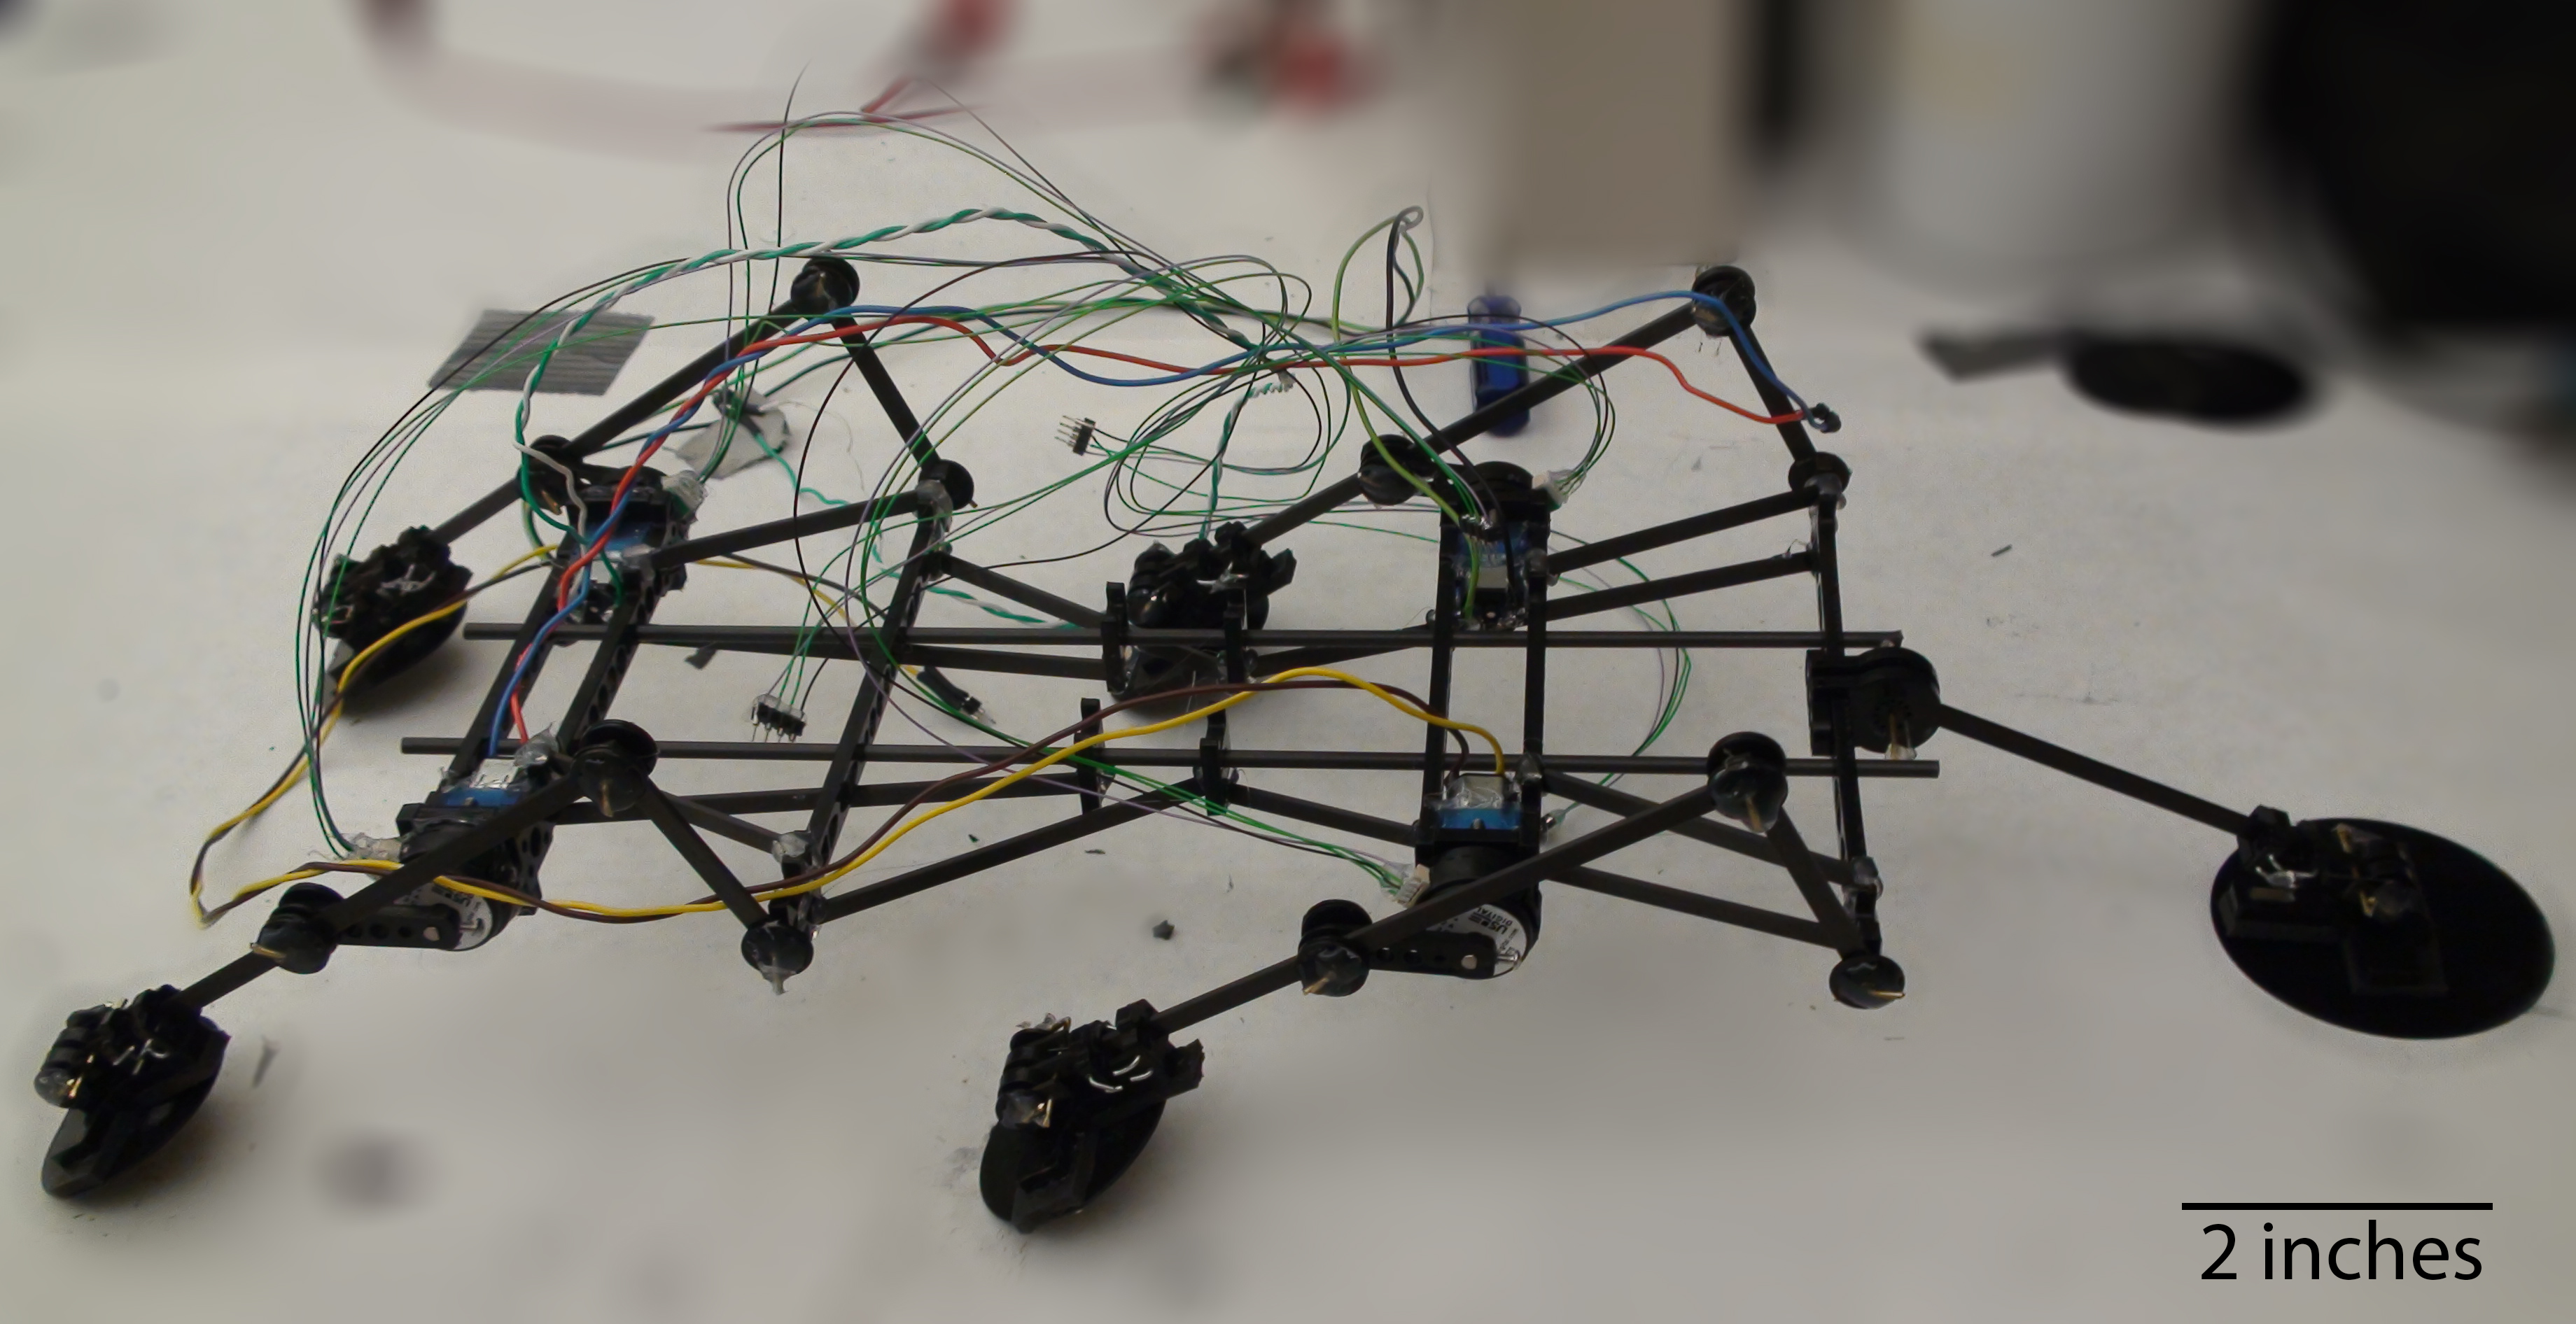
\includegraphics[height = 3.25in]{robot.JPG}
    \caption{Current Robot Hardware.}
	\label{fig:robot}
\end{subfigure}
\quad
\begin{subfigure}[t]{0.47\textwidth}
    \centering
    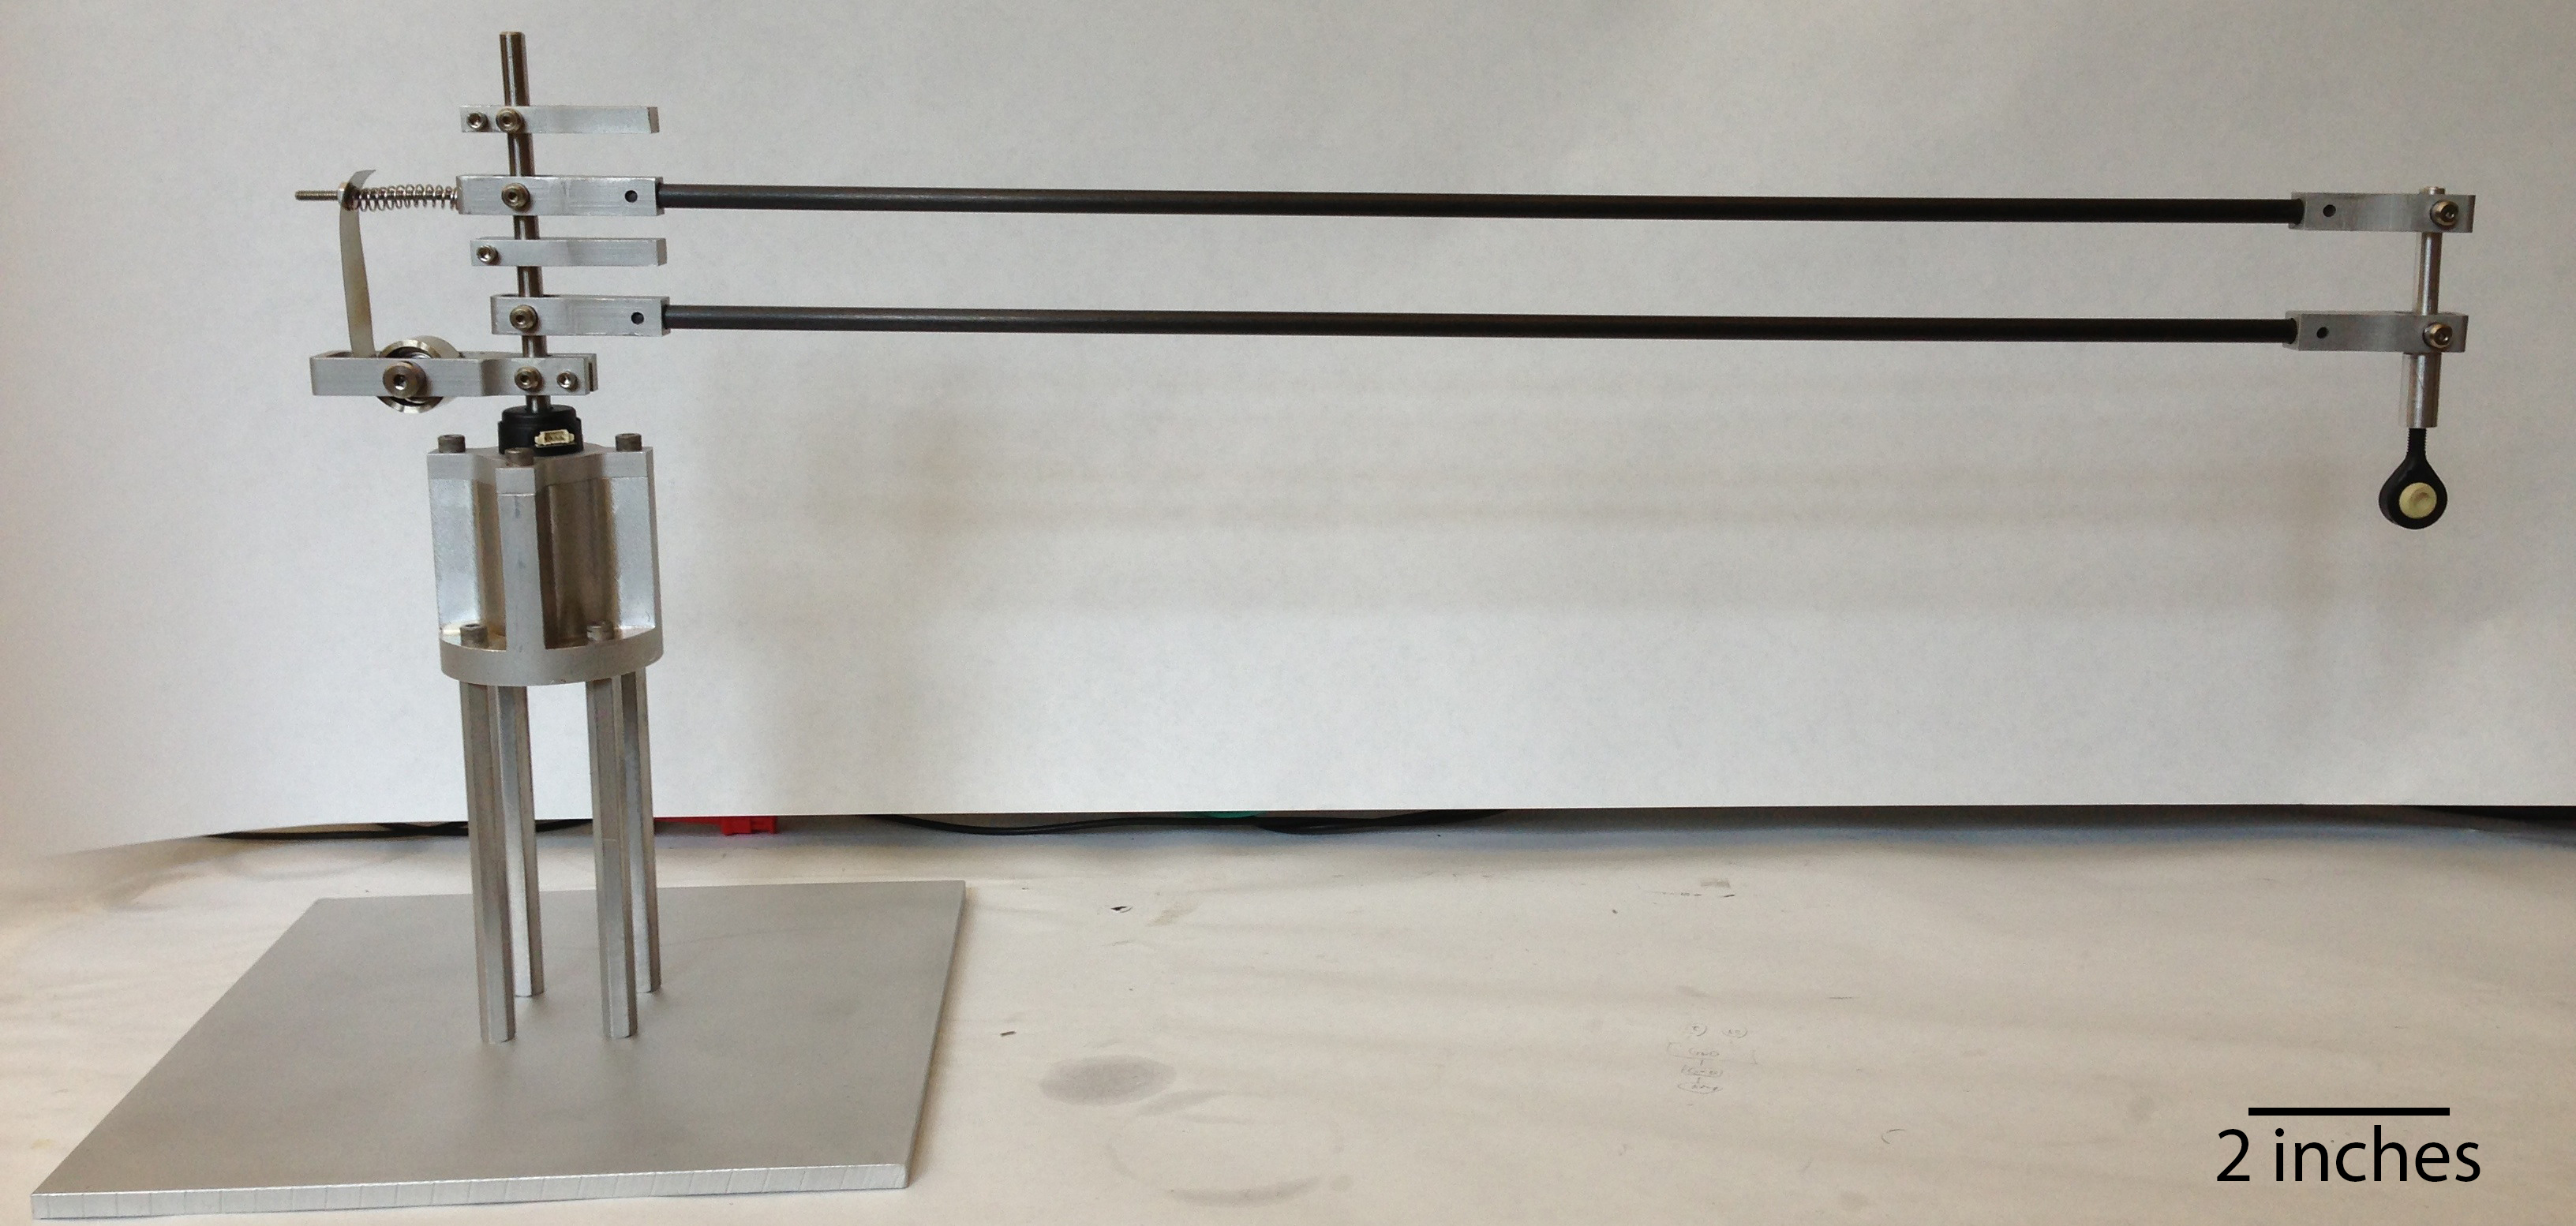
\includegraphics[height = 3.25in]{boom.jpg}
    \caption{Testing Boom}
	\label{fig:boom}
\end{subfigure}
\vspace{0.5EX}
\caption{Rotating boom setup will allow us to test the robot as it runs in a circle in a small pool.} 
\label{fig:test}
\end{figure}
